%! TEX root = thesis.tex

\chapter{Results and Discussion}%
\label{sec:results}

In this particular chapter, we will be looking at the results that have been captured through the experiments conducted to improve the baselines. The results from the experiments along with the baseline have been consolidated in Table \ref{consolidated-results-summary}. The baseline metrics from the zero evaluation studies are grayed out to differentiate between the baseline and new experiments. Additionally, all experiments have a symbol associated with them as seen in the first column of the table. This will be used to represent the corresponding experiment when looking at a comparative analysis of the Validation Word Error Rate (WER) across the experiments as seen in Figure \ref{fig:experiment-wers}.

\section{Experiment Results}%
\label{sec:results}

As seen from the Table \ref{consolidated-results-summary}, the best result is obtained from the experiment where fine-tuning (transfer learning) and Singing Voice Separation(SVS) has been applied to the Whisper model. This enables the Whisper model to leverage the speech representations it already has learnt to be adapted to the songs domain. Additionally, fine-tuning for Whisper also improves the decoding procedure as the model is able to better adapt to the lyrics domain. This represents an improvement of 0.31 WER (or 57.4\% improvement) over the baseline Whisper architecture that was showcased. The second best results are seen in the implementation of fine-tuning (transfer learning) with the Wav2Vec2 architecture as an encoder and Connectionist Temporal Classification (CTC) with beam search and 5-gram lyrics language model (see Figure \ref{fig:lyricslanguagemodel} ) as the decoder. This represents an improvement of 0.36 WER (or 60\% improvement) over the baseline Wav2Vec2 architecture.


\renewcommand{\arraystretch}{2}
\setlength{\arrayrulewidth}{0.3mm}
\begin{table}[H]
\small
\begin{center}
\begin{tabular}{ |p{1.5cm} | p{1cm} | p{6cm}| p{2cm}| p{2cm}| p{1cm}| }
\multicolumn{6}{c}{ } \\
\cline{1-6}
\textbf{Symbol} & \textbf{Input} & \textbf{Models}  & \textbf{Decoder} & \textbf{LM} & \textbf{WER}  \\
\hline  \hline
\textcolor{gray}{M1} & \textcolor{gray}{Music} & \textcolor{gray}{\textit{Wav2Vec2 Large Self (Zero Shot)}} & \textcolor{gray}{Greedy} & \textcolor{gray}{None} & \textcolor{gray}{0.96}  \\
\textcolor{gray}{M2} & \textcolor{gray}{Music}  & \textcolor{gray}{\textit{Whisper Large (Zero Shot)}} & \textcolor{gray}{Transformer} &  \textcolor{gray}{None} & \textcolor{gray}{0.85} \\
\hline
V3 & Vocal & \textit{Wav2Vec2 Large Self (Zero Shot)} & Greedy &  None & 0.85  \\
V4 & Vocal  & \textit{Whisper Large (Zero Shot)} & Transformer &  None & 0.68 \\
\hline
F5 & Vocal & \textit{Wav2Vec2 Large Self (Fine-tuned)} & Greedy &  None & 0.74  \\
F6 & Vocal  & \textit{Whisper Large (Fine-tuned)} & Transformer &  None & 0.61 \\
\hline
L7 & Vocal & \textit{Wav2Vec2 Large Self (Fine-tuned)} & Beam &  5gram & \underline{0.60}  \\
L8 & Vocal  & \textit{Whisper Large (Fine-tuned)} & Transformer &  PostProcess & \textbf{0.54} \\
\hline
T9 & Vocal & \textit{Wav2Vec2 Large Self (Fine-tuned)} & Transformer &  BERT & 0.83  \\
T10 & Vocal & \textit{Whisper Large (Encoder only)} & Transformer &  BERT & 0.82  \\

 \hline  \hline
\end{tabular}
\caption{\label{consolidated-results-summary} Songs to Lyrics Transcription Experiment Results \\ \textit{Top Result is shown with a Bold value and the Second best is shown with an underline}}
\end{center}
\end{table}

The Figure \ref{fig:experiment-wers} shows the convergence of the different experiments across their run of the experiments. The plot shows the evolution of the evaluation metric, Word Error Rate, across the epochs of the corresponding experiments. The graph is normalized as a percentage of the total number of epochs to have a comparative view of how the experiments stack up to one another. The first observation is that all models converge to their equilibrium as can be seen by the flat tail of the Word Error Rate metrics in the model. Additionally, when looking at the experiments that are differentiated with only the language model, we can see that there is an improvement of 7 - 13\% in the model. Another observation is that there is only a marginal improvement in the encoder-decoder architecture implemented.

In subsequent sections, we will cover key questions and analysis from the results we have just shared.


\begin{figure}
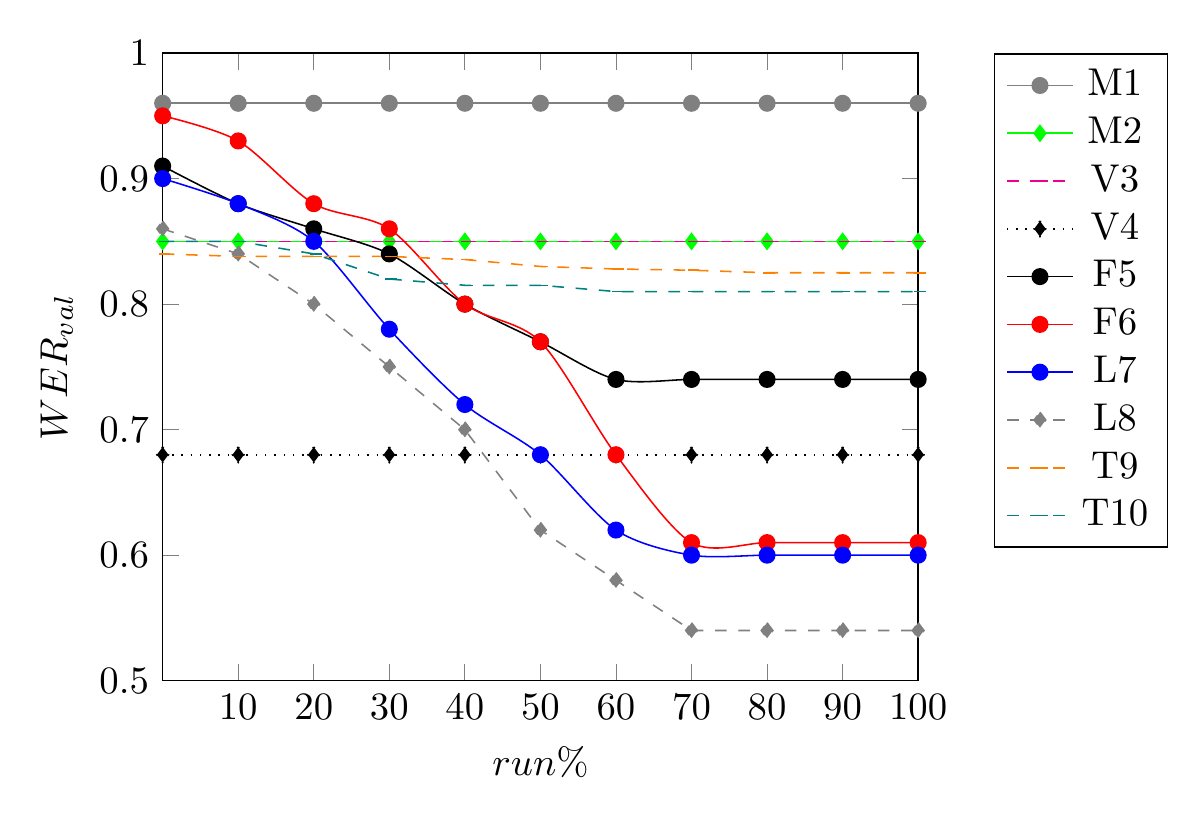
\begin{tikzpicture}[scale=1.4]
    \begin{axis}[
        legend style={at={(1.1,1)},anchor=north west},
        xlabel=$run \%$,
        ylabel=$WER_{val}$,
        xmin=0, xmax=100,
        ymin=0.5, ymax=1,
        xtick={10,20,30,40,50,60,70,80,90,100},
        ytick={0.50,0.60,0.70,0.80,0.90,1.0}
        ]
    \addplot[smooth,mark=*,gray] plot coordinates {
        (0,0.96)
        (10,0.96)
        (20,0.96)
        (30,0.96)
        (40,0.96)
        (50,0.96)
        (60,0.96)
        (70,0.96)
        (80,0.96)
        (90,0.96)
        (100,0.96)
    };
    \addlegendentry{M1}

    \addplot[solid,mark=diamond*,green] plot coordinates {
        (0,0.85)
        (10,0.85)
        (20,0.85)
        (30,0.85)
        (40,0.85)
        (50,0.85)
        (60,0.85)
        (70,0.85)
        (80,0.85)
        (90,0.85)
        (100,0.85)
    };
    \addlegendentry{M2}

    \addplot[dashed,mark=-,magenta] plot coordinates {
        (0,0.85)
        (10,0.85)
        (20,0.85)
        (30,0.85)
        (40,0.85)
        (50,0.85)
        (60,0.85)
        (70,0.85)
        (80,0.85)
        (90,0.85)
        (100,0.85)
    };
    \addlegendentry{V3}

    \addplot[dotted,mark=diamond*,black] plot coordinates {
        (0,0.68)
        (10,0.68)
        (20,0.68)
        (30,0.68)
        (40,0.68)
        (50,0.68)
        (60,0.68)
        (70,0.68)
        (80,0.68)
        (90,0.68)
        (100,0.68)
    };
    \addlegendentry{V4}

    \addplot[smooth,mark=*,black] plot coordinates {
        (0,0.91)
        (10,0.88)
        (20,0.86)
        (30,0.84)
        (40,0.80)
        (50,0.77)
        (60,0.74)
        (70,0.74)
        (80,0.74)
        (90,0.74)
        (100,0.74)
    };
    \addlegendentry{F5}

        \addplot[smooth,mark=*,red] plot coordinates {
        (0,0.95)
        (10,0.93)
        (20,0.88)
        (30,0.86)
        (40,0.80)
        (50,0.77)
        (60,0.68)
        (70,0.61)
        (80,0.61)
        (90,0.61)
        (100,0.61)
    };
    \addlegendentry{F6}

    \addplot[smooth,mark=*,blue] plot coordinates {
        (0,0.90)
        (10,0.88)
        (20,0.85)
        (30,0.78)
        (40,0.72)
        (50,0.68)
        (60,0.62)
        (70,0.60)
        (80,0.60)
        (90,0.60)
        (100,0.60)
    };
    \addlegendentry{L7}

    \addplot[dashed,mark=diamond*,gray] plot coordinates {
        (0,0.86)
        (10,0.84)
        (20,0.80)
        (30,0.75)
        (40,0.70)
        (50,0.62)
        (60,0.58)
        (70,0.54)
        (80,0.54)
        (90,0.54)
        (100,0.54)
    };
    \addlegendentry{L8}


    \addplot[dashed,mark=-,orange] plot coordinates {
        (0,0.84)
        (10,0.838)
        (20,0.838)
        (30,0.838)
        (40,0.8355)
        (50,0.83)
        (60,0.828)
        (70,0.827)
        (80,0.825)
        (90,0.825)
        (100,0.825)
    };
    \addlegendentry{T9}

    \addplot[dashed,mark=-,teal] plot coordinates {
        (0,0.85)
        (10,0.85)
        (20,0.84)
        (30,0.82)
        (40,0.815)
        (50,0.815)
        (60,0.81)
        (70,0.81)
        (80,0.81)
        (90,0.81)
        (100,0.81)
    };
    \addlegendentry{T10}


    \end{axis}
    \end{tikzpicture}
    \caption{Validation Word Error Rates (WER) across experiments} \label{fig:experiment-wers}
    \end{figure}




\subsection{\textbf{  Why is the Encoder-Decoder architecture not improving the baseline?}}

The Encoder - decoder architecture is implemented by using Wav2Vec2 or the Whisper Encoder only model as the encoder and BertLM as the decoder. The outputs from the encoder are the hidden states of the model that is passed along with a sequence of lyrics for the training to work (with teacher forcing). This is already explained in Section \ref{sec:experiments}. We can analyze the training process by removing the \texttt{EarlyStopping} and seeing how longer training of the encoder-decoder module affects the model run. As it can be seen in Figure \ref{fig:encoder-decoder-loss-curves}, the validation losses remain mostly around the same (even with a slight increase) but the training losses keep dropping. This shows that there is an overfitting that is happening as the model is training further. This is a problem that has been seen with Transformer based architectures as seen here -  \cite{mosbach2020stability} and \cite{devlin2018bert}. The main reason for the instability as per the papers shared above is to increase the dataset size with increased diversity to overcome this. We will cover this in the Future Direction and next steps part.

\begin{figure}
     \begin{subfigure}[b]{0.48\textwidth}
         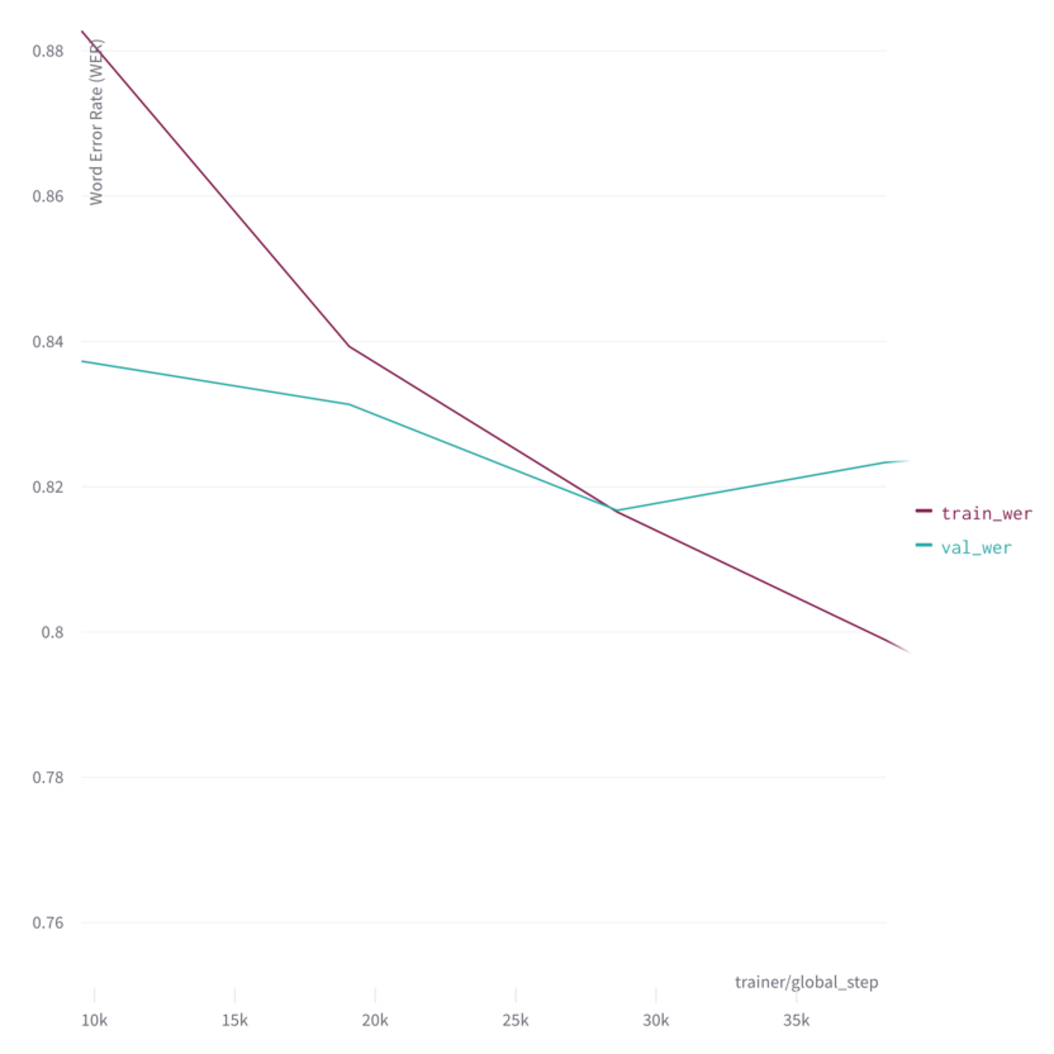
\includegraphics[width=\textwidth]{05-research study/figures/wav2vec2-bert-wer-graph.pdf}
         \caption{Wav2Vec2 Encoder - BertLM Decoder}
         \label{fig:wav2vec2-bert}
     \end{subfigure}
     \hfill
     \begin{subfigure}[b]{0.48\textwidth}
         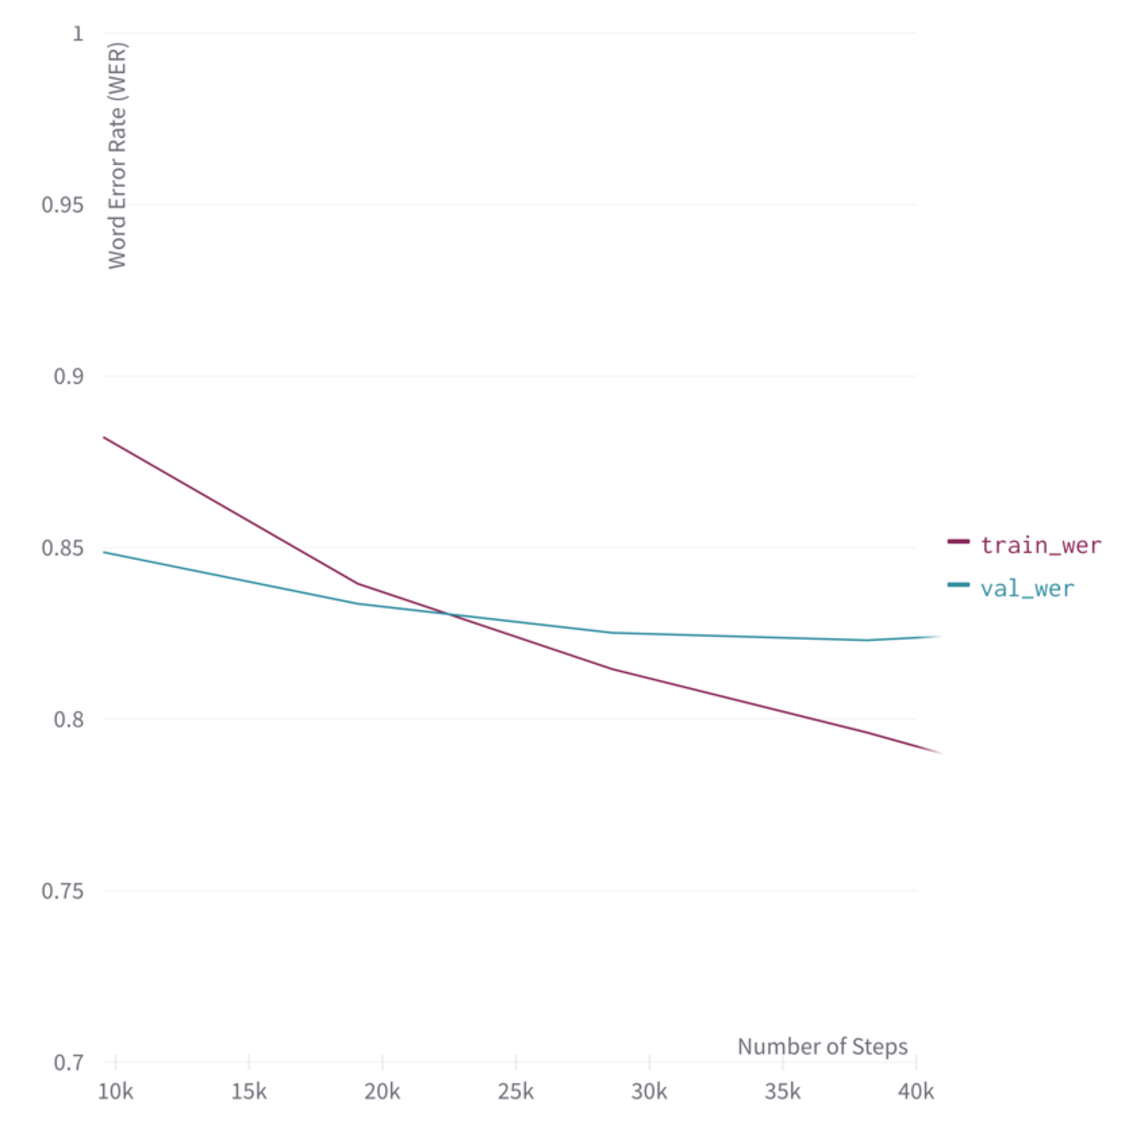
\includegraphics[width=\textwidth]{05-research study/figures/whisper-bert-wer-graph.pdf}
         \caption{Whisper Encoder - BertLM Decoder}
         \label{fig:whisper-bert}
     \end{subfigure}
     \hfill
        \caption{Loss Curves with \texttt{EarlyStopping=False}}
        \label{fig:encoder-decoder-loss-curves}
\end{figure}

\subsection{\textbf{ Error Analysis of results from Greedy and Beam Search with 5-gram Language Model}}

Beam Search with Language models improves the greedy results. While we can see the improvement from the metric, let us see some illustrations on how Wav2Vec2 with the 5-gram KenLM language model improves the prediction and where it doesn't.

The most common area where we see the beam search with language model improving on the greedy search is when the greedy search is able to paint a rough picture of the lyrics but is not able to syntactically make the predicton correct. At these instants, the beam search and language model provide a mechanism to correct and reframe the lyrics. For example, let us take one audio snippet where the lyrics are \texttt{SO LEARN FROM YOUR MISTAKES}. When predicting using Greedy Search, we get the result \texttt{SO LEARNFROMYOURMISTAKES}. By using the language model, we can see that the prediction is corrected to \texttt{SO LEARN FROM YOUR MISTAKE}. Similarly, for the true lyrics of \texttt{ CLOSING TIME OPEN ALL THE DOORS}, greedy search prediction is \texttt{CLOSINGTIMEOPEN ALLTHEDOORS}. The language model corrects the prediction to \texttt{CLOSING TIME OPEN ALL THE DOOR}. .

On the other case, when the Wav2vec2 model is not able to generate the right features from the audio snippet, the beam search does not provide the correct lyrics. To illustrate, let us take the example of \texttt{ONE TWO ONE TWO THREE ARGHH}, greedy search predicts \texttt{TOO} and beam search with language model predicts \texttt{O}. In this case, the model is not able to transcribe the true lyrics at all.

We can see from visual inspection that the beam search with language model improves the readability aspect of the results. For example, let us take the lyrics \texttt{YOU LEAVE ME ONCE AGAIN HOME ALONE}, greedy search based decoder predicts \texttt{VERY WIM TAKIN ON MY DOTER} and beam search with language model predicts \texttt{VERY I'M TAKING ON MY DATE}. While the transcribed lyrics are wrong in this case, it definitely is more readable for the user.

\subsection{\textbf{What are the common errors seen in the best performing model?}}

The best model is the Fine-tuned Whisper Model with DEMUCS applied to the audio signal and post-processing done on the outputs. The details on the post-processing can be seen in \ref{sec:experiments}.The results from the Whisper model are confident but not always correct. However, the results from the model are readable and well formed.To illustrate, the Whisper model transcribes accurately on most of the scenarios covered by the Wav2Vec2 model shown in the previous section. For the true lyrics of \texttt{so learn from your mistakes}, Whisper predicts correct \texttt{so learn from your mistakes}. When Whisper makes mistakes, it confidently makes mistakes. Take this example - \texttt{you leave me once again home alone}. Whisper predicts it as \texttt{the only one taking all my own}. Similarly, taking a common example shared for the Wav2Vec2 model, let us take the lyrics \texttt{one two one two three arghh}, Whisper predicts \texttt{so what you want to know}.

Hence, it can be seen that while the Word Error Rates are in the 53-54\% range , the readability of the model results are good. While it depends on the problem, this can be a positive (Lyrics Generation task) or negative feature (Lyrics Transcription).


\begin{figure}
    \centering
    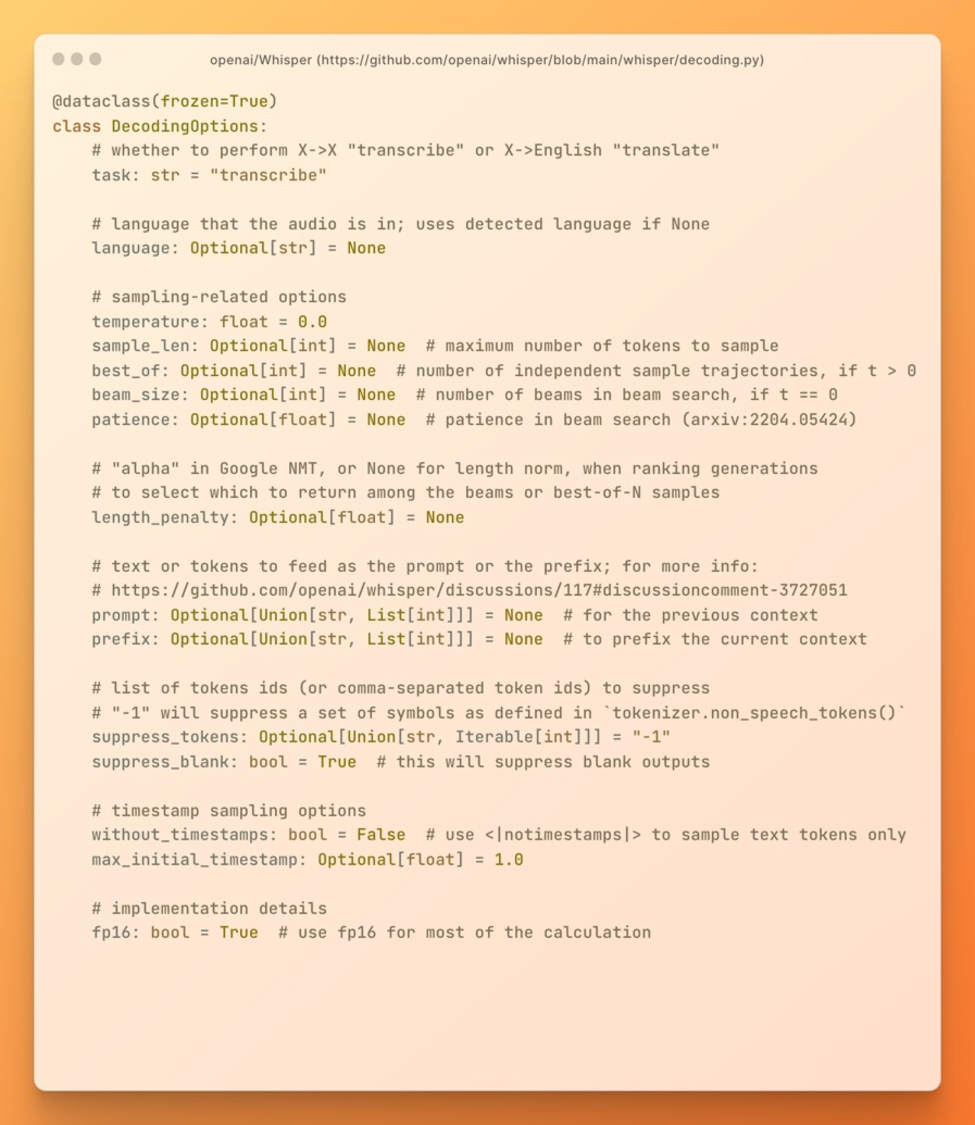
\includegraphics[width=0.9\textwidth]{05-research study/figures/whisper-decoder-code-snippet.pdf}
    \caption{Whisper Decoder Code Snippet}
    \label{fig:whisper-code-snippet}
\end{figure}


To deep dive into it, we can take a look into the code-base from Open AI's Whisper model. Whisper has a sophisticated decoder architecture that includes language identification, temperature controlled sampling techniques, beam search, prompting and prefixing \cite{radford2023robust}. Additionally, the decoder part of the encoder-decoder architecture with the additional features such as prompting etc. give Whisper the ability to generate text better than a N-grams language model (It uses Transformers architecture as a language model).

\section{Discussion}

Till this chapter, we have looked at the problem statement and how it can be applied to commercial products, the theoretical concepts behind the thesis, formulation of the problem statement, experimentation and results with analysis and discussion about some of the key questions that come from the thesis study. In the next chapter, we will focus on concluding the study with giving a summary of the conclusion of answering the research questions framed at the beginning of the thesis. We will then summarize the results and pave the way towards future steps and direction with this research direction.
